\begin{exercice}[Divisibilité par 4 et 100]
Un nombre est divisible par 4 si et seulement si le nombre formé par ses deux derniers chiffres est divisible par 4.\\[0.5em]
Un nombre est divisible par 100 si et seulement si ses deux derniers chiffres sont 0.\\[0.5em]
Parmi les nombres

21 ; 12 ; 2 ; 619 ; 120 ; 416 ; 296 ; 540 ; 1700,

quels sont les nombres divisibles par :
\begin{colenumerate}{2}
 \item 4 ?
 \item 100 ?
 \end{colenumerate}
\end{exercice}


\begin{exercice}[Pair]
Explique pourquoi le produit de deux entiers consécutifs est toujours pair.
\end{exercice}


\begin{exercice}[Séminaire]
Lors d'un séminaire, 324 personnes doivent se répartir dans divers ateliers. Tous les ateliers doivent avoir le même effectif, compris entre 30 et 60 personnes. Quelles sont les différentes possibilités ?
\end{exercice}


\begin{exercice}[Nombres parfaits]
\begin{enumerate}
 \item Écris la liste de tous les diviseurs de 6 ;
 \item Calcule la somme de tous ces diviseurs à l'exception de 6 ;
 \item Que remarques-tu ? On appelle nombre parfait tout entier qui a cette particularité ;
 \item Vérifie que 496 est un nombre parfait ;
 \item Trouve tous les nombres parfaits compris entre 20 et 30.
 \end{enumerate}
\end{exercice}


\begin{exercice}
Trouve les nombres entiers de trois chiffres multiples de 5 dont la somme des chiffres est 21.
\end{exercice}


\begin{exercice}[Les trois filles]
Dans une famille, il y a trois filles. La somme de leurs âges est 13 et le produit est 36.

Quel est l'âge de chaque fille ? Trouve toutes les possibilités.
\end{exercice}


\begin{exercice}[Pages]
Deux livres ont respectivement 160 et 192 pages. Chacun de ces livres est formé de fascicules ou cahiers, qui ont tous un même nombre de pages, compris entre 30 et 50.
\begin{enumerate}
 \item Quel est le nombre de pages d'un cahier ?
 \item Quel est le nombre de cahiers qui composent les deux livres ?
 \end{enumerate}
\end{exercice}


\begin{exercice}[Tempête]
Des poteaux téléphoniques étaient plantés le long d'une route, sur une ligne droite et régulièrement espacés d'un nombre entier de mètres. \\[0.5em]
Après une tempête, il n'en reste plus que trois : le premier et le dernier puis un autre situé entre les deux, à 345 m du premier et 184 m du dernier. Un technicien arrivé sur les lieux estime le nombre de poteaux tombés à plus de 10 mais à moins de 100 ! Combien de poteaux sont-ils tombés ?
\end{exercice}

\begin{exercice}[Arbres]
Un terrain rectangulaire a pour dimensions 168 m et 294 m. Sur ses côtés, on veut planter des arbres régulièrement espacés d'un nombre entier de mètres. Il doit y avoir un arbre à chaque coin du terrain. \\[0.5em]
Quel est le nombre minimum d'arbres que l'on pourra planter ?
\begin{center} 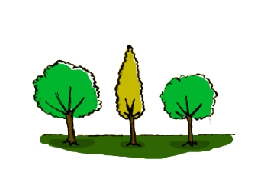
\includegraphics[width=3.3cm]{arbres} \end{center}
\end{exercice}


\begin{exercice}[Piscine]
Une piscine rectangulaire mesure 3,36 m par 7,80 m et a une profondeur de 1,44 m. On désire la carreler avec des carreaux carrés tous identiques. Le carreleur ne veut pas faire de découpes de carreaux mais préfère les grands carreaux, plus faciles à poser. Son fournisseur a toutes les tailles de carreaux en nombre entier de centimètres.
\begin{enumerate}
 \item Quelle taille de carreaux doit-il commander ? Prendre la plus grande mesure possible.
 \item Son fournisseur vend les carreaux par lot de 100. Combien de lots doit-il commander ?
 \end{enumerate}
\end{exercice}


\begin{exercice}[Sacrée collection !]

\vspace{1em}

\begin{minipage}[c]{0.65\linewidth}
Abdel dit à Doris : « J'ai plus de 400 DVD mais moins de 450 !

En les groupant par 2 ou par 3 ou par 4 ou par 5, c'est toujours la même chose, il m'en reste un tout seul ! ».
 \end{minipage} \hfill%
 \begin{minipage}[c]{0.32\linewidth}
  \begin{center} 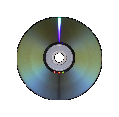
\includegraphics[width=1.4cm]{CD} \end{center}
  \end{minipage} \\
Combien Abdel a-t-il de DVD ?
\end{exercice}


\begin{exercice}[Escalier]
Le nombre de marches d’un escalier est compris entre 40 et 80 :
\begin{itemize}
 \item Si on compte ces marches deux par deux, il en reste une ;
 \item Si on les compte trois par trois, il en reste deux ;
 \item Si on les compte cinq par cinq, il en reste quatre.
 \end{itemize}
Quel est le nombre de marches de cet escalier ?
\end{exercice}


\begin{exercice}[La numération moderne]
$3 \cdot 10^3 + 2 \cdot 10^2 + 8 \cdot 10^1 + 4 \cdot 10^0$ est la décomposition en base « dix » de 3\,284. Décompose les nombres 5\,348 et 4\,367 \,214 en base « dix ».
\end{exercice}


\begin{exercice}[Les limites de la calculatrice]
\begin{enumerate}
 \item Avec la calculatrice, donne un ordre de grandeur du produit de 987\,654 par 876\,534 ;
 \item Calcule le résultat exact de ce produit.
 \end{enumerate}
\end{exercice}


\begin{exercice}[L'unité d'enregistrement informatique]
En informatique, on utilise une unité d'enregistrement appelée « octet ».
\begin{enumerate}
 \item Calcule avec ta calculatrice la valeur des expressions suivantes :
 \begin{itemize}
  \item $A = 2^{10}$ octets ;
  \item $B = 2^{20}$ octets ;
  \item $C = 2^{30}$ octets.
  \end{itemize}
 \item Explique pourquoi l'expression $A$ est généralement appelée « 1 kilooctet ». On note $A \approx 1$ ko ($10^3$ octets). Par approximation, on écrit $A = 1$ ko.
 \item De même $B$ est appelé « 1 Mégaoctet » (1 Mo) et $C$ « 1 Gigaoctet » (1 Go). Indique par quelles puissances de 10, se traduisent les préfixes « méga » et « giga ». 
 \end{enumerate}
\end{exercice}


\begin{exercice}[Multiple et diviseur]
\begin{enumerate}
 \item À l'aide de la calculatrice retrouve les nombres entiers positifs non nuls $n$, $m$ et $p$ tels que :
 
 \begin{center} $349\,272 = 2^n \cdot 3^m \cdot 7^p \cdot 11$ \end{center}

 \item À l'aide de la calculatrice retrouve les nombres entiers positifs non nuls $r$, $s$ et $t$ tels que :
 
 \begin{center} $36\,288 = 2^r \cdot 3^s \cdot 7^t$ \end{center}
 
 \item On considère : $N = 2^3 \cdot 3^3 \cdot 7$.
 
Sans calculer la valeur de $N$, montre que $N$ est un diviseur commun à 349\,272 et à 36\,288.

 \item On considère : $M = 2^6 \cdot 3^4 \cdot 7^2 \cdot 11$.
 
Sans calculer la valeur de $M$, montre que $M$ est un multiple commun à 349\,272 et à 36\,288.
 \end{enumerate}
\end{exercice}


\begin{exercice}[Chemin de diviseurs \ldots]
\begin{center} 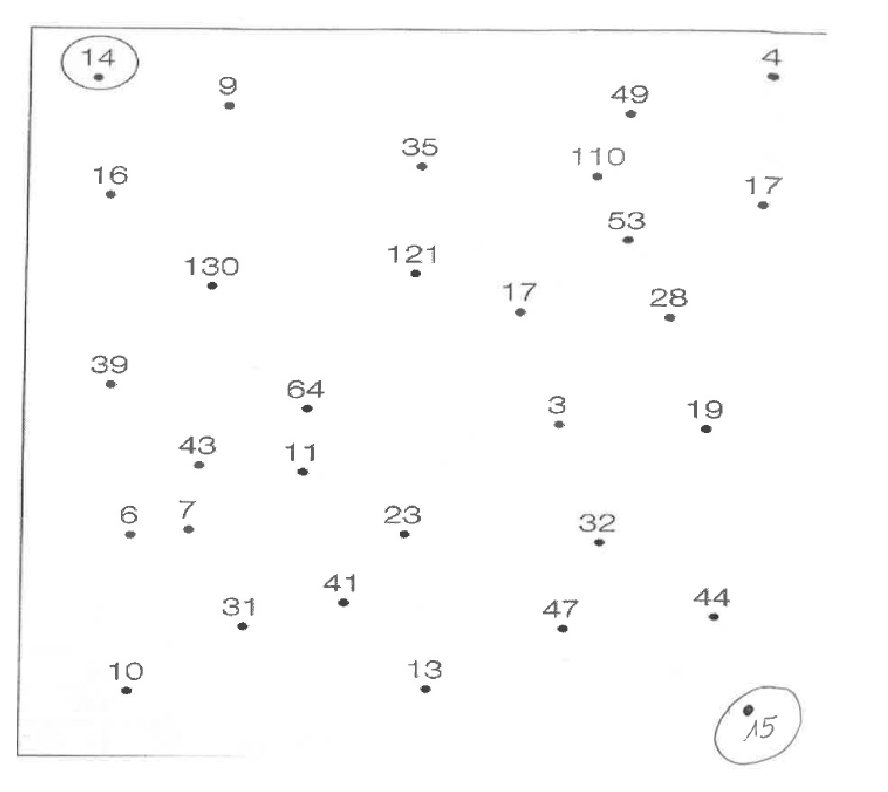
\includegraphics[width=6.9cm]{chemin} \end{center}

Sur la figure ci-dessous, trouver un chemin qui mène de 14 à 15 en alternant multiples et diviseurs. Pour vous aider, continuer le raisonnement suivant : \\[1em]
Je relie 14 à 28 car 28 est un multiple de 14 ;

Je relie 28 à \ldots \ldots car \ldots \ldots est un diviseur de 28 ;

Je relie \ldots à \ldots \ldots car \ldots \ldots est un multiple de \ldots \ldots ;

Je relie \ldots à \ldots \ldots car \ldots \ldots est un diviseur de \ldots \ldots ;

Je relie \ldots à \ldots \ldots car \ldots \ldots est un multiple de \ldots \ldots ;

Je relie \ldots à \ldots \ldots car \ldots \ldots est un diviseur de \ldots \ldots ;

Je relie \ldots à \ldots \ldots car \ldots \ldots est un multiple de \ldots \ldots ;

Je relie \ldots à \ldots \ldots car \ldots \ldots est un diviseur de \ldots \ldots ;

Je relie \ldots à \ldots \ldots car \ldots \ldots est un multiple de \ldots \ldots ;

Je relie \ldots à \ldots \ldots car \ldots \ldots est un diviseur de \ldots \ldots ;

Je relie \ldots à 15 car \ldots \ldots est un multiple de 15.

Tous les nombres du tableau ne sont pas utilisés.

\end{exercice}


\begin{exercice}[Chemin premier \ldots]
Trouver le chemin qui mène de la case $X$ à la case $Y$ en passant par 13 cases (sans compter les cases $X$ et $Y$) contiguës différentes contenant chacune un nombre premier.

\begin{center} 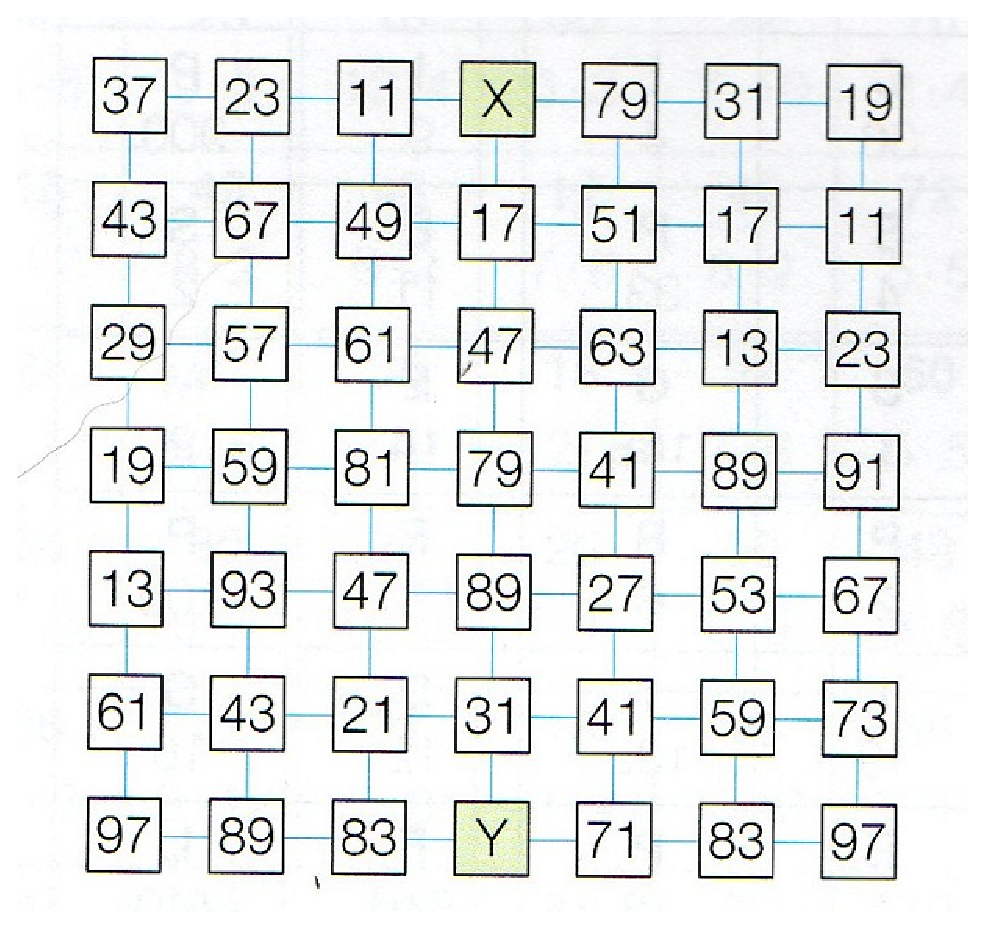
\includegraphics[width=6.5cm]{cheminXY} \end{center}

\begin{center} 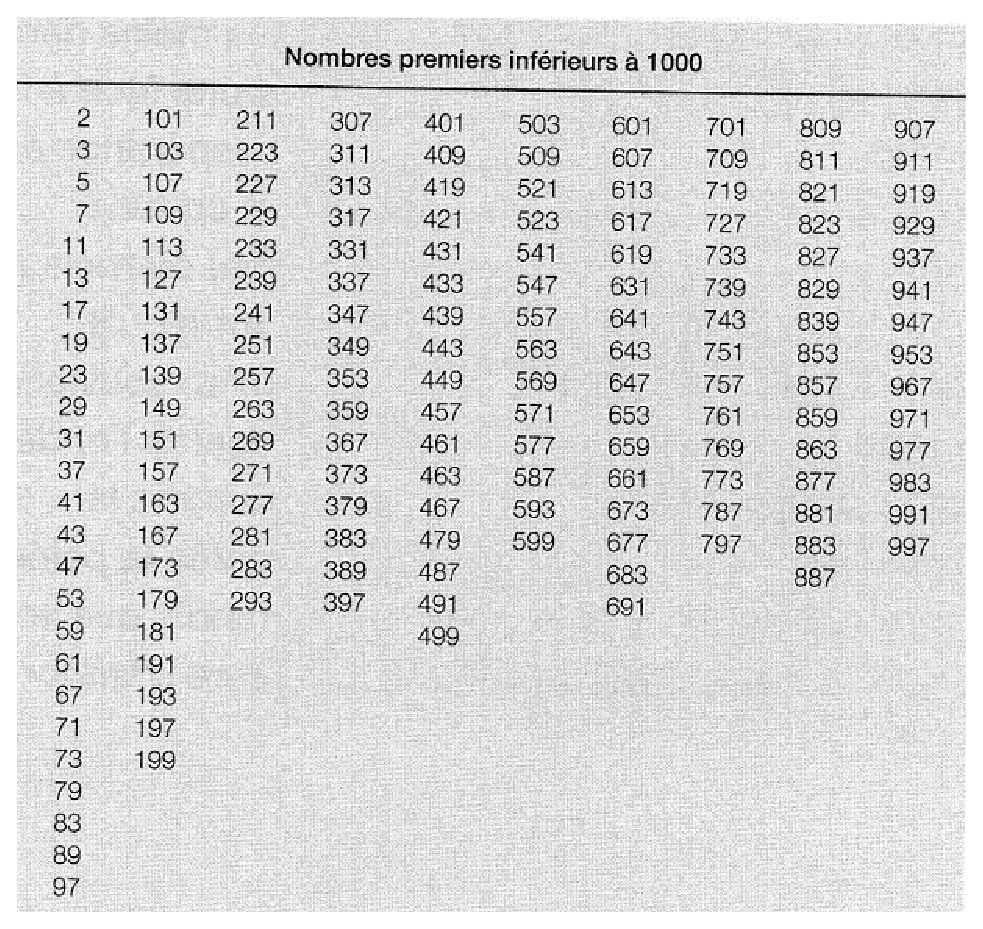
\includegraphics[width=6.6cm]{tableau} \end{center}
\end{exercice}
